\section{Transformation Geometry}

\subsection{Symmetries and Groups}

\defn{Transformation}{
    A continuous bijection \(T: \bR^2 \to \bR^2\) with a continuous inverse is called a (plane)-transformation.
}

\defn{Symmetries}{
    If \(\Gamma\) is a geometric object in the plane, the transformations that preserve (key aspects of) \(\Gamma\) are called symmetrics of \(\Gamma\).
}

\defn{Groups}{
    A group is a non-empty set \(G\) on which a binary operation \(\star\) is defined, such that the following properites hold:
    \begin{enumerate}[label=\alph*)]
        \item Closure: if \(a, b \in G\) then \(a \star b \in G\).
        \item Associativity: if \(a, b, c \in G\) then \((a \star b) \star c) = a \star (b \star c)\).
        \item Identity element: there is an element \(e\) of \(G\) such that for all \(a \in G\) we have \(a \star e = e \star a = a\)
        \item Inverses: for each \(a\) in \(G\) there is an element \(b\) of \(G\) such that \(a \star b = b \star a = e\). This element is usually denoted \(a^{-1}\).
    \end{enumerate}
}

\defn{Abelian Groups}{
    A group \(G\) is abelian if the operation is commutative: \(a \star b = b \star a\) for all \(a, b \in G\).
}

It is easy to see that the set of all transformations of the plane is a group under composition.
\begin{enumerate}[label=\alph*)]
    \item If \(T, S: \bR^2 \to \bR^2\) are continuous bijections, so is \(T \circ S\), and it has continuous inverse \(S^{-1} \circ T^{-1}\).
    \item If \(T, S, U: \bR^2 \to \bR^2\) are any maps on \(\bR^2\), \((T \circ S) \circ U = T \circ (S \circ U)\).
    \item The identity map is a transformation.
    \item We have built into the definition the fact that the inverse of a transformation is also a transformation.
\end{enumerate}

Notation: \(\mathcal{G}_2\) represents the group of all transformations in the plane.

\defn{Subgroup}{
    Let \(G\) be a group, and let \(H\) be a subset of \(G\) which is itself a group (under the same operation as \(G\)). Then we say that \(H\) is a subgroup of \(G\).
}

\lem{The Subgroup Lemma}{
    Let \(G\) be a group and \(H\) a non-empty subset of \(G\). Then \(H\)is a subgroup of \(G\) if and only if it is closed under the group operation and inverse.
}

\begin{corollary}
    The set of symmetries of a geometric figure is a group.
\end{corollary}

\subsection{Affine Transformations}

\defn{Affine Transformation}{
    A transformation \(T \in \mathcal{G}_2\) is an affine transformation or an affinity if it maps lines to lines.
}

Obvious examples of affinities are translations \(\fx \to \fx + \mathbf{b}\) for fixed \(\mathbf{b}\), and reflections in a line.

\begin{theorem}
    The set of all affinities in the plane, \(\mathcal{A}_2\), is a group under composition.
\end{theorem}

\begin{theorem}
    A transformation \(T \in \mathcal{A}_2\) if and only if it is of the form
    \[T(\fx) = A\fx + \mathbf{b}\]
    for a fixed invertible matrix \(A\) and constant vector \(\mathbf{b}\).
\end{theorem}

\begin{theorem}
    Let \(T\) be an affinity.
    \begin{enumerate}[label=\alph*)]
        \item \(T\) will preserve collinearity, concurrence, parallelism, betweenness, line segments, polygons and the ratio of distances on the same or parallel lines.
        \item \(T\) will in general not preserve angles, areas or circularity.
    \end{enumerate}
\end{theorem}

\textit{Proof.}
\begin{itemize}
    \item For collinearity, suppose \(A, B\) and \(C\) are collinear points and \(\ell\) the line through them. Then \(T(\ell)\) is also a line by definition and clearly it goes through \(T(A), T(B)\) and \(T(C)\).
    \item For concurrence, if \(\ell\) and \(\lambda\) are two lines and \(P = \ell \cap \lambda\) then \(T(P) = T(\ell) \cap T(\lambda)\).
    \item For parallelism, if \(\ell\) and \(\lambda\) are parallel lines but \(P = T(\ell) \cap T(\lambda)\) is not empty, then \(T^{-1}(P) \in \ell \cap \lambda = \emptyset\), contradiction.
    \item Let \(T(\fx) + Ax + \fb\).
          \begin{itemize}
              \item Suppose \(R\) lies between \(P\) and \(Q\), so that \(\mathbf{r} = \mathbf{p} + \lambda(\mathbf{q} - \mathbf{p}) \text{ with } \lambda \in (0, 1)\). Then \(T(\mathbf{r}) = A\mathbf{p} + \fb + \lambda(A\mathbf{q} - A\mathbf{p})\), and so \(T(R)\) is between \(T(P) = A\mathbf{p} + \fb\) and \(T(Q) = A\mathbf{q} + \fb\).
          \end{itemize}
    \item It follows from the previous part that \(T\) preserves line segments and hence polygons.
    \item Since we now know \(T\) preserves the order of points on a line, we only need to check the ratio of undirected distances.
          \begin{itemize}
              \item Suppose \(P\) and \(Q\) lie on a line \(\ell\) which we write as \(\fa + \lambda \fc\). Let \(\fp + \fa + t\fc\) and \(\fq + \fa + s\fc\), so \(|PQ| = |t - s| \cdot \norm{\fc}\). If \(P' = T(P)\) and \(Q' = T(Q)\), then \(\fp' = A\fa + \fb + tA\fc\) and \(\fq' = A\fa + \fb + sA\fc\), so that \(|P'Q'| = |t - s| \cdot \norm{A\fc}\).
              \item Likewise for a pair \(U, V\) on \(\ell\) or a line parallel to \(\ell\), we might get \(|UV = |\tau - \sigma| \cdot \norm{\fc}\) and \(|U'V'| = |\tau - \sigma| \cdot \norm{A\fc}\).
              \item So
                    \[\frac{|PQ|}{|UV|} = \frac{|t - s|}{|\tau - \sigma|} = \frac{|P'Q'|}{|U'V'|},\]
                    and the ratio of distances is preserved.
          \end{itemize}
    \item To prove that \(T\) may not preserve angles, areas and circularity, we need only consider an example, such as \(T(\fx) =\begin{pmatrix}
              1 & 1 \\ 0 & 2
          \end{pmatrix}\fx\).
\end{itemize}

Clearly then, an affinity can be thought of as a linear map composed with a translations which is continuous and differentiable. In fact, as an affinity is invertible it is a change of coordinates. From several variable calculus the Jacobian of that coordinate change gives us how transform. \\

It is easy to check that the Jacobian of \(\fx \mapsto A\fx + \fb\) is simply \(|\det(A)|\), and so we have proved:
\begin{theorem}
    An affinity \(T(\fx) = A\fx + \fb\) multiplies areas of geometric figures by \(|\det(A)|\).
\end{theorem}

\defn{Equiareal}{
    A transformation that preserves area is called equiareal.
}

Clearly, equiareal affinities have \(\det(A) = \pm 1\).

\defn{Positive Angle}{
    The angle between the lines \(AB\) and \(AC\) taken in that order and the implied direction is positive if
    \[\det(\fx \mid \fy) = \det\begin{pmatrix}
            x_1 & y_1 \\ x_2 & y_2
        \end{pmatrix} > 0 \text{ for } \overrightarrow{AB} = \begin{pmatrix}
            x_1 \\ x_2
        \end{pmatrix}, \overrightarrow{AC} = \begin{pmatrix}
            y_1 \\ y_2
        \end{pmatrix}.\]
}

Under the affinity \(T(\fx) = A\fx + \fb\), the determinant used to define the orientation of the angle will be simply multiplied by \(\det(A)\). \\

So if \(\det(A) > 0\) the orientation is preserved: we call such affinities \textbf{direct}. If the orientation of angles is reversed the affinity is \textbf{indirect}.

\subsubsection{Applications of Affinities}

\begin{theorem}
    Let \(\ell_1\) and \(\ell_2\) be two lines in \(\bR^n\). There is an affinity \(T\) such that \(T(\ell_1) = \ell_2\).
\end{theorem}

\textit{Proof.} Write the equations of the lines as \(\fx + \lambda \fp + \fb\) and \(fx = \lambda \fq + \fc\) for suitable vectors \(\fp, \fq, \fb\) and \(\fc\). We can easily find an invertible matrix \(A\) such that \(A\fp = \fq\), and then the affinity
\[T(\fx) = A\fx + \fc - A\fb\]
maps the first line to the second. \\

\begin{theorem}
    For any two sets of three non-collinear points \(\{P, Q, R\}\) and \(\{P', Q', R'\}\) in \(\bR^2\) there is a unique affinity \(T\) such that \(T(P) = P', T(Q) = Q'\) and \(T(R) = R'\).
\end{theorem}

Then to summarise the previous two results we say that \textit{all lines} and \textit{all triangles} are \textbf{affinely equivalent}.

\begin{theorem}
    A non-trivial conic section is affinely equivalent to one of the following \textbf{standard forms}:
    \begin{enumerate}[label=\roman*)]
        \item \(x^2 + y^2 = 1\) for an ellipse;
        \item \(x^2 - y^2 = 1\) for a hyperbola;
        \item \(y = x^2\) (or, equivalently, \(x = y^2\)) for a parabola;
        \item \(x^2 = y^2\) for intersecting lines;
        \item \(x^2 = 1\) (or, equivalently, \(y^2 = 1\)) for parallel lines;
        \item \(x = 0\) for one line.
    \end{enumerate}
    Furthermore, the coordinates in which the conic takes its standard form are orthogonal.
\end{theorem}

\thrm{Pascal's Theorem (1639)}{
    Let \(A_1, A_2, A_3, A_4, A_5\) and \(A_6\) be six points on an ellpise \(\mathcal{C}_1\). let \(P_1 = A_1 A_2 \cap A_4 A_5, P_2 = A_2 A_3 \cap A_5 A_6\) and \(P_3 = A_3 A_4 \cap A_6 A_1\)be the points where opposite sides of the hexagon \(A_1 A_2 A_3 A_4 A_5 A_6\) intersect. Then (assuming all three points exists) \(P_1, P_2\) and \(P_3\) are collinear.
    \begin{center}
        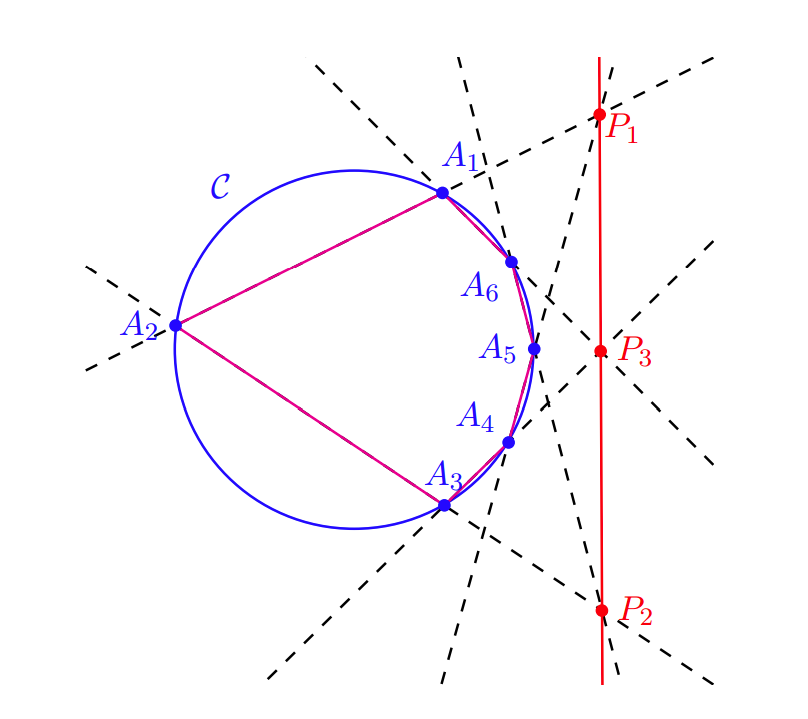
\includegraphics{assets/transformation/pascal.png}
    \end{center}
}

\begin{lemma}
    Let \(\mathcal{C}_1\) and \(\mathcal{C}_2\) be two circles that intersect at \(M\) and \(N\). Let \(AB\) be any chord of \(\mathcal{C}_1\) and \(C, D\) be the second intersections of \(AM\)and \(BN\) respectively with \(\mathcal{C}_2\), as shown. Then \(AB\) and \(CD\) are parallel.
    \begin{center}
        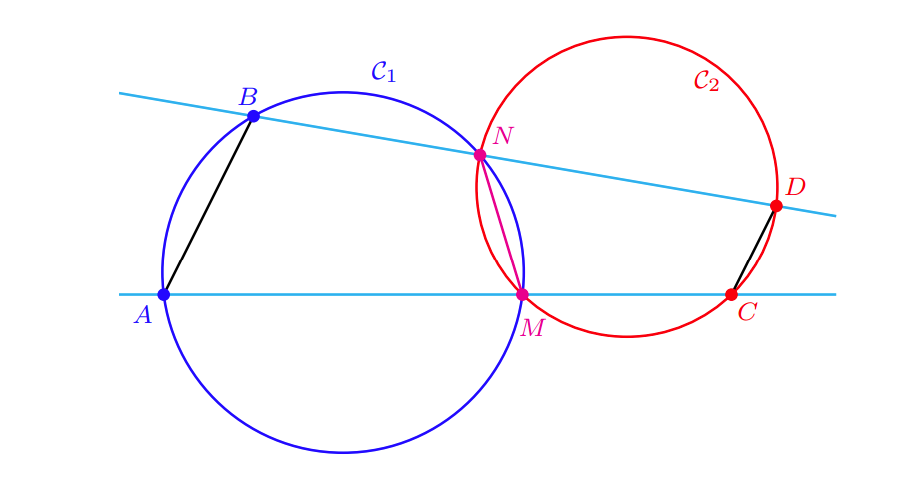
\includegraphics{assets/transformation/lemma_pascal.png}
    \end{center}
\end{lemma}

\subsection{Isometries}

Let \(d: \bR^2 \times \bR^2 \to \bR\) be the usual (Euclidean) distance. If \(A = (a, b)\) and \(B = (c, d)\) in some Cartesian coordinate system,
\[d(A, B) = \sqrt{(a - c)^2 + (b - d)^2}.\]

\defn{Isometry}{
    An isometry, \(T\), is a transformation of the plane that preserves distance:
    \[d(T(A), T(B)) = d(A, B) \text{ for all } A, B \in \bR^2.\]
}

\defn{Congruent}{
    Two figures \(F_1, F_2\) in the plane are congruent if there is an isometry mapping one to the other.
}

\begin{theorem}
    The set of isometries under composition is a subgroup of \(\mathcal{A}_2\) and is denoted \(\mathcal{I}_2\).
\end{theorem}

\begin{theorem}
    An isometry \(T\) preserves betweenness, collinearity, parallelism, line segments, triangles, and polygons. It also preserves
    \begin{enumerate}[label=\roman*)]
        \item the standard dot product on \(\bR^2\);
        \item (sizes of) angles;
        \item circles and conic sections.
    \end{enumerate}
\end{theorem}

\textit{Proof.} The first of properties follows because an isometry is an affinity, but could be easily proved directly.
\begin{enumerate}[label=\roman*)]
    \item Use the polarisation identity \(4(\fx \cdot \fy) = \norm{\fx + \fy}^2 - \norm{\fx - \fy}^2\).
    \item This follows from (i).
    \item Circles  are loci a fixed distance from some central point \(O\), and conic sections are loci of points \(P\) such that for some point \(F\) (the focus), the ratio \(PF / d\) is constant, where \(d\) is the distance of \(P\) from some fixed line (the directrix).
\end{enumerate}

\begin{theorem}
    An affinity \(T\) of the form \(T(\fx) = A\fx + \fb\) is an isometry if and only if \(A\) is orthogonal, i.e. \(A^TA = I\).
\end{theorem}

\subsubsection{Direct Isometries}

\defn{Direct Isometries}{
    An isometry is direct if it preserves orientation of angles. An isometry that reverses the orientation of angles is called indirect.
}

\begin{proposition}
    The set of direct isometries form a group.
\end{proposition}

The set of indirect isometries is not a group, as it is not closed under composition. Additionally, it does not contain the identity.

\defn{Translation}{
    A translation \(T_\fa: \bR^2 \to \bR^2\) is a map defined by \(T_\fa(\fx) = \fx + \fa\).
}

\begin{theorem}
    The set of translations is an abelian group of direct isometries under composition.
\end{theorem}

\defn{Rotation}{
    A rotation through angle \(\theta\) about the origin of coordinates is given by
    \[U_\theta(\fx) = \begin{pmatrix}
            \cos \theta & -\sin \theta \\
            \sin \theta & \cos \theta
        \end{pmatrix}\fx\]
    in cartesian coordinates. It is thus a linear map on \(\bR^2\).
}

\begin{theorem}
    Both the set of translations and set of rotation about the origin form abelian subgroups of direct isometries under composition.
\end{theorem}

\begin{definition}
    A rotation through angle \(\theta\) about a point \(P\) will be denoted \(R_{\theta, P}\).
\end{definition}

\begin{theorem}
    A rotation through angle \(\theta\) about a point \(P\) is a direct isometry given by
    \[R_{\theta, P} = T_\fp \circ U_\theta \circ T_{-\fp}.\]
\end{theorem}

\begin{theorem}
    An affinity \(T\) of the plane of the form \(T(\fx) = A\fx + \fb\), is a rotation if and only if \(A\) is an orthogonal matrix with determinant 1. If the rotation is not trivial (\(A \neq I\)) it has a single fixed point with positive vector \(\fp = (I - A)^{-1}\fb\), and the angle of the rotation is \(\theta\) where \(A = U_\theta\) by the rotation definition.
\end{theorem}

\defn{Displacement}{
    An isometry is called a displacement if it is either a rotation or a translation.
}

\begin{theorem}
    A displacement that has no fixed points is a non-trivial translation; rotations fix exactly one point or all points. Furthermore:
    \begin{enumerate}[label=\roman*)]
        \item The composition of two rotations is either a rotation or a translation.
        \item The composition of a rotation and a translation is a rotation through the same angle.
        \item The set of all displacement is a group under composition.
    \end{enumerate}
\end{theorem}

\begin{theorem}
    Given two pairs of points \(A, B\) and \(A', B'\) with \(d(A, B) = d(A', B')\) there is exactly one direct isometry \(T\) such that \(T(A) = A'\) and \(T(B) = B'\), and it is a displacement.
\end{theorem}

\begin{corollary}
    Every direct isometry is a displacement.
\end{corollary}

\subsubsection{Indirect Isometries}

\defn{Reflection}{
    The transformation \(R_\ell\) is a reflection in the line \(\ell\) if for all \(P\), if \(P' = R_\ell(P), PP'\) is orthogonal to \(\ell\) and \(d(P, M) = d(P', M)\) where \(M = PP' \cap \ell\).
}

\begin{theorem}
    Let \(R_\ell\) be a reflection in a line \(\ell\). Then
    \begin{enumerate}[label=\roman*)]
        \item \(R_\ell \circ R_\ell = R_\ell^2\) is the identity.
        \item \(R_\ell(P) = P\) if and only if \(P \in \ell\).
        \item \(R_\ell\) is an indirect isometry.
        \item If \(\lambda\) is a line perpendicular to \(\ell\) then \(R_\ell(\lambda) = \lambda\).
    \end{enumerate}
\end{theorem}

\begin{theorem}
    Let \(R_\ell\) and \(R_\lambda\) be reflections in the lines \(\ell\) and \(\lambda\) respectively.
    \begin{enumerate}[label=\roman*)]
        \item \(R_\lambda \circ R_\ell\) is a displacement.
        \item If \(\ell\) and \(\lambda\) are parallel then \(R_\lambda \circ R_\ell = T_{2\fa}\), where \(\fa\) is the vector displacement from \(\ell\) to \(\lambda\).
        \item If \(X = \ell \cap \lambda\) exists and \(\theta\) is the (signed) angle from \(\ell\) to \(\lambda\) then \(R_\lambda \circ R_\ell = R_{2\theta, X}\).
    \end{enumerate}
\end{theorem}

\begin{lemma}
    Let \(A\) be a real orthogonal \(2 \times 2\) matrix with determinant \(-1\). Then \(A^2 = I\), \(A\) has eigenvalues \(1\) and \(-1\) and so is diagonalisable.
\end{lemma}

\begin{theorem}
    An affinity \(T\) on \(\bR^2\) of the form \(T(\fx) = A\fx + \fb\), is a reflection if and only if \(A\) is an orthogonal matrix with determinant \(-1\) and \(A\fb = -\fb\). The line of reflection has parametric vector form \(\fx = \lambda\fu + \frac{1}{2}\fb\) where \(\fu \cdot \fb = 0\).
\end{theorem}

\begin{proposition}
    Any rotation can be written as the product of two reflections.
\end{proposition}

\defn{Glide Reflection}{
    An isometry formed from a reflection followed by an arbitrary translation is called a glide reflection.
}

\begin{theorem}
    Given two pairs of points \(A, B\) and \(A', B'\) with \(d(A, B) = d(A', B')\) there is exactly one indirect isometry \(T\) such that \(T(A) = A\) and \(T(B) = B'\), and it is a glide reflection.
\end{theorem}

\begin{corollary}
    Every indirect isometry is either a reflection or a glide reflection.
\end{corollary}

\subsubsection{Summary and a Criterion}

To summarise, any isometry must be of the form \(T(\fx) = A\fx + \fa\) with \(A\) orthogonal (\(A^TA = I\)) and \(\fa\) fixed (possible zero).

\begin{center}
    \begin{tabular}{|c|c|c|c|c|}
        \hline
        Name                   & Type     & \(\det(A)\) & Fixed points/lines & Invariant points/lines          \\
        \hline
        \hline
        translation by \(\fb\) & direct   & 1           & none               & lines parallel to \(\fb\)       \\
        \hline
        rotation around \(P\)  & direct   & \(1\)       & \(P\)              & none (unless half or full turn) \\
        \hline
        reflection in \(\ell\) & indirect & \(-1\)      & \(\ell\)           & lines orthogonal to \(\ell\)    \\
        \hline
        glide reflection       & indirect & \(-1\)      & none               & one line                        \\
        \hline
    \end{tabular}
\end{center}

\begin{theorem}
    An isometry is determined by its effect on three non-collinear points.
\end{theorem}

\subsection{Similarities}

A similarity is a transformation that preserves shape but no necessarily size.

\defn{Similarity}{
    A transformation \(T: \bR^2 \to \bR^2\) is a similarity if there is a constant \(k > 0\) such that \(d(T(A), T(B)) = kd(A, B)\) for all \(A, B \in \bR^2\). The constant \(k\) is the same for every \(A\) and \(B\), and is known as the ratio of \(T\).
}

If we are paying heed to the direction of lines, then we would allow \(k < 0\) too. A similarity scales all lengths in all directions the same: it is an \textbf{isotropic scaling}. Similarities with \(k > 0\) are also called \textbf{dilatations} or \textbf{dilations}. If the origin is preserved a similarity is sometimes called a \textbf{homothety}.

\defn{Similar}{
    If \(F_1\) and \(F_2\) are geometric objects related by a similarity we say they are similar.
}

\begin{theorem}
    The set of Similarities under composition is a subgroup of \(\mathcal{A}_2\) and denoted \(\mathcal{SM}_2\). Also the set of isometries, \(\mathcal{I}_2\) is a subgroup of \(\mathcal{SM}_2\).
\end{theorem}

\begin{theorem}
    A similarity \(S\) preserves betweenness, concurrence, collinearity, line segments, triangles, polygons, (sizes of) angles, circles, ellipses (or any conic section), parallelism and ratios of distances.
\end{theorem}

\begin{theorem}
    A similarity is determined by its effect on three non-collinear points.
\end{theorem}

\defn{Radial Transform}{
    A radial transform with centre \(P\) and ratio \(k \neq 0\) is the map \(D_{k, P}\) given by
    \[D_{k, P}(\fx) = k(\fx - \fp) + \fp = k\fx + (1 - k)\fp.\]
    \begin{center}
        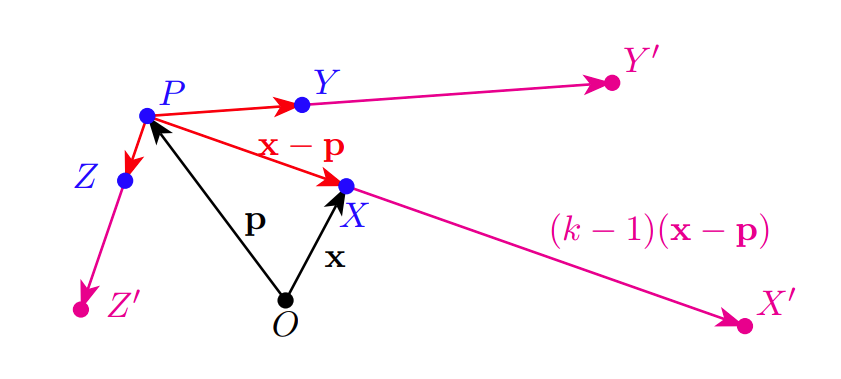
\includegraphics{assets/transformation/radial_transform.png}
    \end{center}
}

\begin{proposition}
    For a fixed point \(P\) the set of radial transforms with centre \(P\) are an abelian subgroup of \(\mathcal{SM}_2\).
\end{proposition}

\begin{theorem}
    Every similarity, \(S\), of ratio \(k\) is of the form \(D_{k, P} \circ T\) for some isometry \(T\) and some point \(P\).
\end{theorem}
